\chapter{Setup}
\usemintedstyle{default}
% \section{Participants}
% \begin{figure}[h]
%     \centering
%     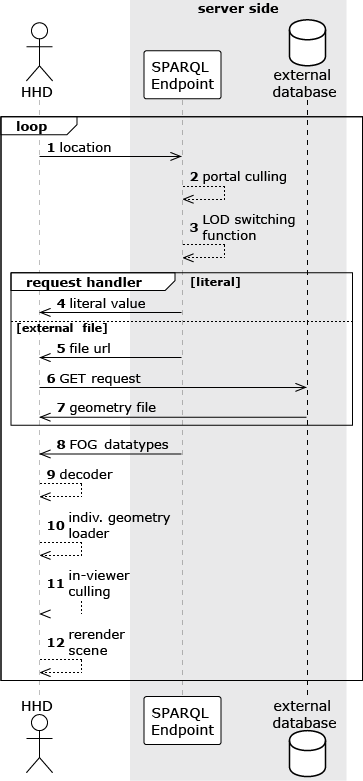
\includegraphics[width=6cm]{./figures/sequenceDiagram.png}
%     \caption{Sequence diagram}
%     \label{fig:sequendeDiagram}
% \end{figure}
% \section{Framework}
% \subsection{Nextjs}
% \section{Querying}
% \subsection{Front-end}
% \subsection{Back-end}
% \section{Rendering}
% \subsection{Xeokit \acs{sdk}}

\section {Pages}
\subsection{index}
\inputminted{tsx}{figures/snippets/src/pages/index.tsx}
\begin{minted}{tsx}
import dynamic from "next/dynamic";
import Head from "next/head";
import { Navbar, Querypannel } from "~/components";

const ARViewer = dynamic(() => import("~/components/ARViewer"), {
  ssr: false,
});

export default function Home() {
  return (
    <>
      <Head>
        <title>Create T3 App</title>
        <meta name="description" content="Generated by create-t3-app" />
        <link rel="icon" href="/favicon.ico" />
      </Head>
      <main>
        <div className="absolute top-14 h-[calc(100vh-3.5rem)] w-full overflow-hidden">
          <ARViewer />
        </div>
        <Navbar />
        <Querypannel/>
      </main>
    </>
  );
}
\end{minted}
\newpage
\section {Components}
\subsection{ARViewer}
\inputminted{tsx}{figures/snippets/src/components/ARViewer.tsx}
\newpage
\subsection{Navbar}
\inputminted{tsx}{figures/snippets/src/components/Navbar.tsx}
\newpage
\subsection{QueryPannel}
\inputminted{tsx}{figures/snippets/src/components/QueryPannel.tsx}

\newpage
\section {Modules}
\subsection{Viewer}
\subsubsection{useInitViewer}
\inputminted{ts}{figures/snippets/src/modules/viewer/useInitViewer.ts}
\newpage
\subsubsection{useLoadGeometry}
\inputminted{ts}{figures/snippets/src/modules/viewer/useLoadGeometry.ts}
\newpage
\subsection{fetchSPARQL}
\inputminted{ts}{figures/snippets/src/modules/fetchSPARQL.ts}
\newpage
\subsection{useCacheManagement}
\inputminted{ts}{figures/snippets/src/modules/useCacheManagement.ts}

The Xeokit \ac{sdk} ...